\subsection{Ensemble Learning -- XGBoost}\label{subsec:ensemble-learning}

\subsubsection{Cơ sở lý thuyết}

\paragraph{1. Nguyên lý học tổ hợp và Mô hình cộng dồn Gradient Boosting}\mbox{}\\
Học tổ hợp (\textit{Ensemble Learning}) là phương pháp kết hợp nhiều mô hình cơ sở (\textit{weak learners}) nhằm tạo ra một bộ dự đoán mạnh hơn và ổn định hơn từng mô hình đơn lẻ. Hai chiến lược phổ biến là \textit{Bagging} (huấn luyện song song nhiều mô hình độc lập để giảm phương sai) và \textit{Boosting} (huấn luyện tuần tự sao cho mỗi mô hình mới tập trung sửa sai cho các mô hình trước đó để giảm độ chệch).

\textbf{XGBoost} (\textit{eXtreme Gradient Boosting}) là biến thể tối ưu hiệu năng cao của thuật toán Gradient Boosted Decision Trees (GBDT). Với tập dữ liệu $N$ mẫu $\{(\mathbf{x}_n, y_n)\}_{n=1}^{N}$ ($\mathbf{x}_n \in \mathbb{R}^D$, $y_n \in \{0, 1\}$), XGBoost biểu diễn điểm dự đoán thô $\hat{z}_n$ dưới dạng tổng cộng dồn của $K$ cây quyết định hồi quy (CART):
\begin{equation}
    \hat{z}_n = \sum_{k=1}^{K} f_k(\mathbf{x}_n), \qquad f_k \in \mathcal{F}
\end{equation}
trong đó $\mathcal{F} = \{f(\mathbf{x}) = w_{q(\mathbf{x})}\}$ là không gian các cây hồi quy, $q(\mathbf{x}) \in \{1, \dots, T\}$ ánh xạ mẫu $\mathbf{x}$ tới chỉ số nút lá tương ứng và $w_j \in \mathbb{R}$ là trọng số của lá $j$. Đối với bài toán phân loại nhị phân, xác suất hậu nghiệm thuộc lớp gian lận $\mathcal{C}_1$ được suy ra qua hàm Sigmoid:
\begin{equation}
    \hat{y}_n \triangleq p(\mathcal{C}_1 \mid \mathbf{x}_n) = \sigma(\hat{z}_n) = \frac{1}{1 + e^{-\hat{z}_n}} \in (0, 1)
\end{equation}
Cơ chế xây dựng cây tuần tự của Gradient Boosting / XGBoost được minh họa tại Hình~\ref{fig:xgboost-boosting}.

\begin{figure}[H]
    \centering
    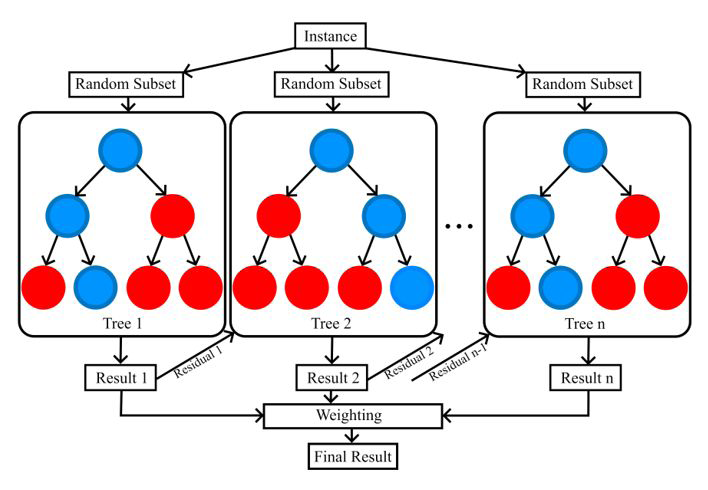
\includegraphics[width=0.80\linewidth]{graphics/xgboost_boosting.png}
    \caption{Minh họa cơ chế xây dựng tuần tự các cây quyết định trong mô hình XGBoost}
    \label{fig:xgboost-boosting}
\end{figure}

\paragraph{2. Hàm mục tiêu có điều chuẩn và Xấp xỉ Taylor bậc hai}\mbox{}\\
Điểm khác biệt cốt lõi giúp XGBoost vượt trội so với Gradient Boosting truyền thống là tích hợp trực tiếp thành phần điều chuẩn độ phức tạp cây $\Omega(f)$ vào hàm mục tiêu. Tại bước lặp thứ $t$, cây mới $f_t$ được bổ sung để cực tiểu hóa:
\begin{equation}
    \mathcal{L}^{(t)} = \sum_{n=1}^{N} l\!\left(y_n, \hat{z}_n^{(t-1)} + f_t(\mathbf{x}_n)\right) + \Omega(f_t), \qquad \Omega(f) = \gamma T + \frac{1}{2}\lambda_{\text{reg}} \sum_{j=1}^{T} w_j^2
\end{equation}
trong đó $l(y_n, \hat{z}_n) = -\left[y_n \log\sigma(\hat{z}_n) + (1 - y_n)\log(1 - \sigma(\hat{z}_n))\right]$ là hàm mất mát Binary Cross-Entropy, $T$ là số nút lá, $\gamma \ge 0$ phạt việc tạo thêm nút lá mới và $\lambda_{\text{reg}} \ge 0$ là hệ số điều chuẩn L2 giúp làm mượt trọng số lá, chống quá khớp.

Áp dụng khai triển Taylor bậc hai quanh $\hat{z}_n^{(t-1)}$ và loại bỏ các hằng số không phụ thuộc vào $f_t$, hàm mục tiêu xấp xỉ thu được có dạng:
\begin{equation}
    \tilde{\mathcal{L}}^{(t)} = \sum_{j=1}^{T} \left[ \left(\sum_{n \in I_j} g_n\right) w_j + \frac{1}{2}\left(\sum_{n \in I_j} h_n + \lambda_{\text{reg}}\right) w_j^2 \right] + \gamma T
\end{equation}
trong đó $I_j = \{n \mid q(\mathbf{x}_n) = j\}$ là tập các mẫu rơi vào nút lá $j$, còn $g_n$ và $h_n$ lần lượt là đạo hàm bậc nhất và bậc hai của hàm mất mát theo $\hat{z}_n^{(t-1)}$:
\begin{equation}
    g_n = \frac{\partial l(y_n, \hat{z}_n^{(t-1)})}{\partial \hat{z}_n^{(t-1)}} = \hat{y}_n^{(t-1)} - y_n, \qquad h_n = \frac{\partial^2 l(y_n, \hat{z}_n^{(t-1)})}{\partial (\hat{z}_n^{(t-1)})^2} = \hat{y}_n^{(t-1)}\big(1 - \hat{y}_n^{(t-1)}\big)
\end{equation}

\paragraph{3. Trọng số lá tối ưu, Tiêu chí chia nhánh (Gain) và Thuật toán Histogram}\mbox{}\\
Đặt $G_j = \sum_{n \in I_j} g_n$ và $H_j = \sum_{n \in I_j} h_n$. Với một cấu trúc cây cố định, nghiệm tối ưu của trọng số lá $w_j^*$ và giá trị hàm mục tiêu tương ứng đạt được bằng cách cho đạo hàm theo $w_j$ bằng $0$:
\begin{equation}
    w_j^* = -\frac{G_j}{H_j + \lambda_{\text{reg}}}, \qquad \tilde{\mathcal{L}}^{(t)*}(q) = -\frac{1}{2}\sum_{j=1}^{T} \frac{G_j^2}{H_j + \lambda_{\text{reg}}} + \gamma T
\end{equation}
Khi xét tách một nút thành hai nhánh trái ($I_L$) và phải ($I_R$), độ giảm mất mát (\textit{Gain}) được tính bằng:
\begin{equation}
    \text{Gain} = \frac{1}{2}\left[\frac{G_L^2}{H_L + \lambda_{\text{reg}}} + \frac{G_R^2}{H_R + \lambda_{\text{reg}}} - \frac{(G_L + G_R)^2}{H_L + H_R + \lambda_{\text{reg}}}\right] - \gamma
\end{equation}
Phép chia nhánh chỉ được chấp nhận khi $\text{Gain} > 0$. Sau khi xây dựng xong cây $f_t$, đóng góp của cây được nhân với tốc độ học $\eta \in (0, 1]$ (\textit{shrinkage}): $\hat{z}_n^{(t)} = \hat{z}_n^{(t-1)} + \eta f_t(\mathbf{x}_n)$ nhằm chừa không gian cho các cây sau tinh chỉnh dần và giảm nguy cơ quá khớp.

Nhằm tối ưu tốc độ trên dữ liệu bảng quy mô lớn, thuật toán chia nhánh theo biểu đồ tần suất (\texttt{tree\_method="hist"}) gom các giá trị đặc trưng liên tục vào các thùng rời rạc (\textit{bins}) và tích lũy tổng $(G, H)$ theo từng thùng (Hình~\ref{fig:xgboost-hist}), kết hợp tính toán song song trên nhiều lõi CPU giúp rút ngắn đáng kể thời gian huấn luyện mà vẫn duy trì độ chính xác cao.

\begin{figure}[H]
    \centering
    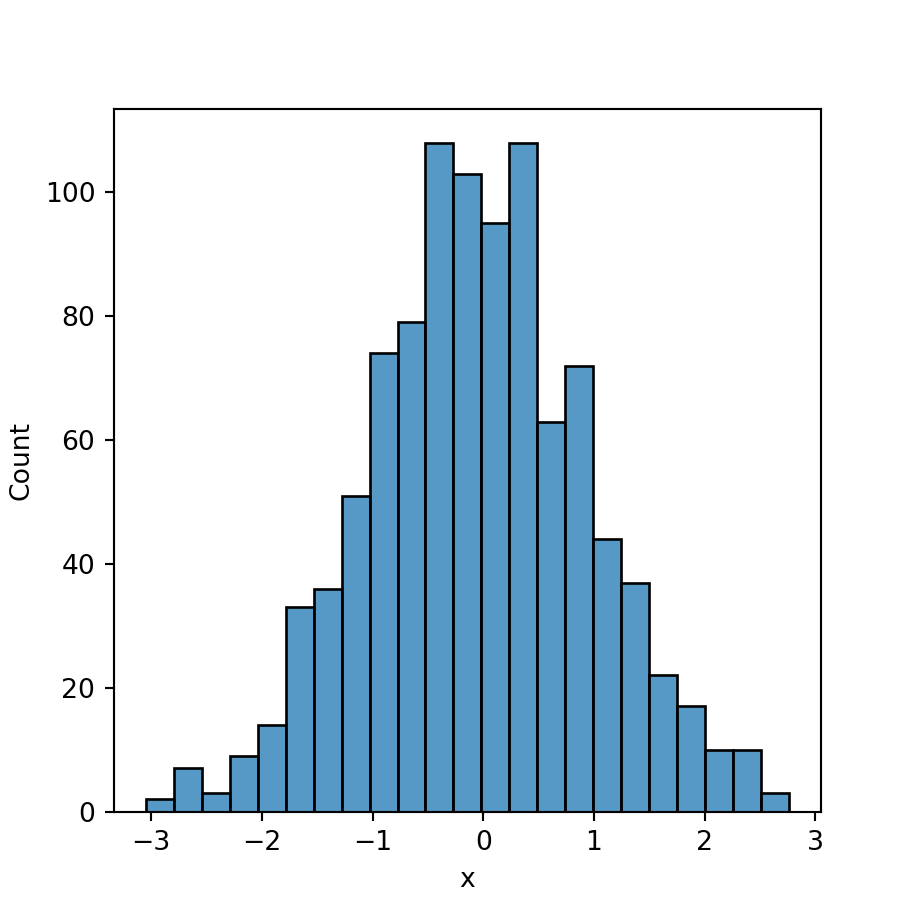
\includegraphics[width=0.78\linewidth]{graphics/xgboost_hist.png}
    \caption{Minh họa kỹ thuật rời rạc hóa đặc trưng theo thùng (\textit{histogram}) để tìm ngưỡng chia nhánh tối ưu trong XGBoost}
    \label{fig:xgboost-hist}
\end{figure}

\subsubsection{Áp dụng mô hình vào bài toán}

\paragraph{1. Môi trường và Thư viện sử dụng}\mbox{}\\
Mô hình được cài đặt bằng ngôn ngữ \textbf{Python} với các thư viện chính:
\begin{itemize}
    \item \texttt{xgboost}: Cung cấp lớp \texttt{XGBClassifier} để xây dựng và huấn luyện mô hình Gradient Boosted Trees hiệu năng cao.
    \item \texttt{scikit-learn}: Cung cấp \texttt{RobustScaler} cho bước chuẩn hóa đặc trưng và \texttt{StratifiedKFold} cho kiểm định chéo phân tầng.
    \item \texttt{NumPy}: Hỗ trợ tính toán mảng và xử lý vector hóa dữ liệu.
\end{itemize}

\paragraph{2. Quy trình tiền xử lý và Huấn luyện}\mbox{}\\
Quy trình thực nghiệm trong tệp \texttt{src/model\_ensemble.py} được đồng bộ với khung đánh giá chung của toàn hệ thống nhằm đảm bảo so sánh công bằng và không rò rỉ dữ liệu (\textit{data leakage}):
\begin{enumerate}
    \item \textbf{Phân chia dữ liệu phân tầng:} Dữ liệu sau tiền xử lý được chia thành tập huấn luyện toàn phần và tập kiểm tra độc lập, kết hợp kiểm định chéo \textit{Stratified K-Fold} để duy trì tỷ lệ giao dịch gian lận nhất quán qua từng \textit{fold}.
    \item \textbf{Chuẩn hóa đồng nhất theo từng fold:} Mặc dù mô hình dựa trên cây quyết định ít nhạy với biến đổi đơn điệu của đặc trưng, các cột thuộc \texttt{COLS\_TO\_SCALE} vẫn được chuẩn hóa bằng \texttt{RobustScaler} riêng biệt trong từng \textit{fold} (\texttt{fit\_transform} trên tập huấn luyện con, \texttt{transform} trên tập kiểm định) để đồng bộ hoàn toàn pipeline tiền xử lý với các mô hình khác.
    \item \textbf{Huấn luyện và Đánh giá:} Mô hình \texttt{XGBClassifier} giữ nguyên phân phối dữ liệu gốc (nhờ khả năng tách vùng phi tuyến mạnh của tổ hợp cây điều chuẩn), thực hiện đánh giá chéo trên 5 \textit{folds}, sau đó huấn luyện lại mô hình cuối cùng trên $100\%$ tập huấn luyện và đánh giá trên tập kiểm tra độc lập với ngưỡng phân loại $\lambda = 0.5$ thông qua mô-đun \texttt{src/metrics.py}.
\end{enumerate}

\paragraph{3. Thiết lập siêu tham số}\mbox{}\\
Cấu hình chi tiết trong hàm \texttt{build\_model()} của tệp \texttt{src/model\_ensemble.py} được tổng hợp tại Bảng~\ref{tab:xgb_hyperparams}.

\begin{table}[H]
\centering
\caption{Thiết lập siêu tham số cho mô hình XGBoost (\texttt{src/model\_ensemble.py})}
\label{tab:xgb_hyperparams}
\renewcommand{\arraystretch}{1.2}
\begin{tabular}{|l|l|p{8.0cm}|}
\hline
\textbf{Siêu tham số} & \textbf{Giá trị} & \textbf{Mục đích sử dụng} \\
\hline
\texttt{n\_estimators} & \texttt{100} & Số lượng cây quyết định được xây dựng tuần tự trong tổ hợp Boosting. \\
\hline
\texttt{learning\_rate} & \texttt{0.1} & Hệ số thu nhỏ ($\eta$) điều tiết đóng góp của từng cây, cân bằng giữa tốc độ hội tụ và chống quá khớp. \\
\hline
\texttt{max\_depth} & \texttt{3} & Giới hạn độ sâu tối đa mỗi cây ở mức nông (3 tầng), kiểm soát độ phức tạp và giảm phương sai. \\
\hline
\texttt{tree\_method} & \texttt{"hist"} & Sử dụng thuật toán chia nhánh dựa trên histogram giúp tăng tốc mạnh trên dữ liệu lớn ($\approx 284$ nghìn mẫu). \\
\hline
\texttt{n\_jobs} & \texttt{-1} & Sử dụng toàn bộ số luồng CPU khả dụng để tính toán song song khi xây dựng cây. \\
\hline
\texttt{random\_state} & \texttt{42} & Cố định hạt giống ngẫu nhiên nhằm đảm bảo tính tái lập kết quả thực nghiệm. \\
\hline
\end{tabular}
\end{table}
